\documentclass[twoside,twocolumn]{article}

\usepackage{blindtext} % Package to generate dummy text throughout this template 
\usepackage{flafter} 
\usepackage{graphicx}
\usepackage[sc]{mathpazo} % Use the Palatino font
\usepackage[T1]{fontenc} % Use 8-bit encoding that has 256 glyphs
\linespread{1.05} % Line spacing - Palatino needs more space between lines
\usepackage{microtype} % Slightly tweak font spacing for aesthetics
\input{arduinoLanguage.tex}

\usepackage[english]{babel} % Language hyphenation and typographical rules

\usepackage[hmarginratio=1:1,top=32mm,columnsep=20pt]{geometry} % Document margins
\usepackage[hang, small,labelfont=bf,up,textfont=it,up]{caption} % Custom captions under/above floats in tables or figures
\usepackage{booktabs} % Horizontal rules in tables

\usepackage{lettrine} % The lettrine is the first enlarged letter at the beginning of the text

\usepackage{enumitem} % Customized lists
\setlist[itemize]{noitemsep} % Make itemize lists more compact

\usepackage{abstract} % Allows abstract customization
\renewcommand{\abstractnamefont}{\normalfont\bfseries} % Set the "Abstract" text to bold
\renewcommand{\abstracttextfont}{\normalfont\small\itshape} % Set the abstract itself to small italic text

\usepackage{titlesec} % Allows customization of titles
\renewcommand\thesection{\Roman{section}} % Roman numerals for the sections
\renewcommand\thesubsection{\roman{subsection}} % roman numerals for subsections
\titleformat{\section}[block]{\large\scshape\centering}{\thesection.}{1em}{} % Change the look of the section titles
\titleformat{\subsection}[block]{\large}{\thesubsection.}{1em}{} % Change the look of the section titles

\usepackage{fancyhdr} % Headers and footers
\pagestyle{fancy} % All pages have headers and footers
\fancyhead{} % Blank out the default header
\fancyfoot{} % Blank out the default footer
\fancyhead[C]{4-Bit Ripple Binary Counter $\bullet$ 13 October 2017} % Custom header text
\fancyfoot[RO,LE]{\thepage} % Custom footer text

\usepackage{titling} % Customizing the title section

\usepackage{hyperref} % For hyperlinks in the PDF

\setlength{\droptitle}{-4\baselineskip} % Move the title up

\pretitle{\begin{center}\Huge\bfseries} % Article title formatting
\posttitle{\end{center}} % Article title closing formatting
\title{4-Bit Ripple Binary Counter} % Article title
\author{%
\textsc{Nakka Chakradhar}\\[1ex] % Your name
%\normalsize IITH \\ % Your institution
\normalsize \href{mailto:ee16tech11022@iith.ac.in}{ee16tech11022@iith.ac.in} % Your email address
\and % Uncomment if 2 authors are required, duplicate these 4 lines if more
\textsc{Adithya Hosapate}\\[1ex] % Second author's name
%\normalsize IITH \\ % Second author's institution
\normalsize \href{mailto:ee16btech11040@iith.ac.in}{ee16btech11040@iith.ac.in} % Second author's email address
\and % Uncomment if 2 authors are required, duplicate these 4 lines if more
\textsc{S Sai Ashish}\\[1ex] % Second author's name
%\normalsize IITH \\ % Second author's institution
\normalsize \href{mailto:ee16btech11043@iith.ac.in}{ee16btech11043@iith.ac.in} % Second author's email address
\and % Uncomment if 2 authors are required, duplicate these 4 lines if more
\textsc{Anand N Warrier}\\[1ex] % Second author's name
%\normalsize IITH \\ % Second author's institution
\normalsize \href{mailto:ee16btech11042@iith.ac.in}{ee16btech11042@iith.ac.in} % Second author's email address
}

\date{\today} % Leave empty to omit a date
\renewcommand{\maketitlehookd}{%
\begin{abstract}
In this project, we made a ripple binary counter using D flip-flops. The binary counter also displays its output on a 7 segment display. We have utilized Verilog for RTL synthesis and simulation of waveforms of 4-bit counter.
\end{abstract}
}

%----------------------------------------------------------------------------------------

\begin{document}

% Print the title
\maketitle

%----------------------------------------------------------------------------------------
%	ARTICLE CONTENTS
%----------------------------------------------------------------------------------------

\section{Introduction}

A binary counter is a hardware circuit that is made out of a series of flip-flops. The output of one flip-flop is sent to the input of the next flip-flop in the series. A binary counter can be either asynchronous or synchronous, depending on how the flip-flops are connected together.

\section{Methods to build}

There are two ways to build a binary counter - synchronous or asynchronous (aka ripple)
\begin{itemize}
\item Synchronous counters are the counters where the clock ports of all flip-flops are multiplexed and are supplied with the same clock signal from the same source
\item Asynchronous counters aka Ripple counters are the counters where the subsequent clock signals are given from the outputs of the previous flip-flops
\end{itemize}

\section{Types of asynchronous counters}

There are three types of asynchronous counter-
\begin{itemize}
	\item n-bit Up-Counter
	\item n-bit Down-Counter
	\item n-bit Up/Down-Counter 
\end{itemize}

\section{Approach}
We built this circuit by adopting the ripple counter concept. To build a 4-bit ripple counter we used the following components   
\begin{table}[htp]
\caption{Components}
\centering
\begin{tabular}{llr}
\toprule
%\multicolumn{2}{c}{Name} \\
%\cmidrule(r){1-2}
Component & Quantity \\
\midrule
D Flip-flops (IC7474) & 2\\
LEDs & $4$ \\
7-Segment diplay & $2$ \\
Arduino Uno & $1$ \\
\bottomrule
\end{tabular}
\end{table}



\subsection{Principle}
Let us assume that the 4 Q outputs of the flip flops are initially 0000. When the rising edge of the clock pulse is applied to the FF0, then the output $Q_{0}$ will change to logic 1 and the next clock pulse will change the $Q_{0}$ output to logic 0. This means the output state of the clock pulse toggles (changes from 0 to 1) for one cycle.

As the $Q'$ of FF0 is connected to the clock input of FF1, then the clock input of second flip flop will become 1. This makes the output of FF1 to be high (i.e. $Q_{0} = 1$), which indicates the value 2. In this way the next clock pulse will make the $Q_{0}$ to become high again.

So now both $Q_{0}$ and $Q_{1}$ are high, this results in making the 4 bit output 0011. Now if we apply the fourth clock pulse, it will make the $Q_{0}$ and $Q_{1}$ to low state and toggles the FF2. So the output $Q_{2}$ will become 0100. As this circuit is 4 bit up counter, the output is sequence of binary values from 0, 1, 2, 3...15 i.e. 0000 to 1111 (0 to 15)

\section{Circuit Diagram}
\begin{figure}[!h]
	\caption{4-bit Ripple Binary counter}
	\includegraphics[width=\linewidth]{Binary-counter.png}
	%\label{fig:boat1}
\end{figure}
%\includegraphics[height=3cm][width=5cm]{Binary-counter.png}.
\section{Working}

\subsection{Ripple effect}

The sum of time delay of individual clock pulses, that drive the circuit is called "Clock ripple".
Each of the previous delays will add to the delay of next flip flop and the sum of all these individual flip flops is known as the propagation delay of circuit.

\section{Method}
In this project we took 4 rising-edge triggered d flip-flops and connected the output of the first flip-flop $(Q')$ to the next flip-flop's clock. This can be extended indefinitely to get an n-bit binary counter.
\newline
As an extension to this module, we used 2 7-segment displays to show the decimal counterpart of the binary number generated by the counter. To show a two digit-number on the segments, we used the concepts of multiplexing and Karnaugh maps to find the boolean expressions for each segment. Also we used an Arduino to display it as the BDC (Binary to decimal decoder) is restricted to decode only till 9(1001)
\subsection{Boolean expressions for segments}   
For the clock signal, we used Arduino to generate it. Also we included a reset button to reset the counter at will (Reset it to 0000).   

The boolean expressions we have used to decode binary numbers to seven segment display can be found in the code below.


\section{Arduino Code}
\subsection{Binary Counter}
	\begin{lstlisting}[frame=single]
	int a,b,c,d,e,f,g;
int led=8,temp;
int current;
int initial;
int pin1=0;
int A=0,B=0,C=0,D=0;

void setup()
{
  pinMode(0,OUTPUT);
  pinMode(1,OUTPUT);
  pinMode(2,OUTPUT);
  pinMode(3,OUTPUT);
  pinMode(4,OUTPUT);
  pinMode(5,OUTPUT);
  pinMode(6,OUTPUT);
  pinMode(7,OUTPUT);
  pinMode(8,OUTPUT);
  pinMode(9,INPUT);
  pinMode(10,INPUT);
  pinMode(11,INPUT);
  pinMode(12,INPUT);
  pinMode(13,OUTPUT);
}



void loop()
{
  digitalWrite(led, HIGH);   
  delay(10);
  digitalWrite(led, LOW);  
  
  A=digitalRead(9);
  B=digitalRead(10);
  C=digitalRead(11);
  D=digitalRead(12);
  /*Serial.print(A);
  Serial.print(B);
  Serial.print(C);
  Serial.print(D);
  
  Serial.print("\n");*/
  
  initial=millis();
  current=initial;
  while (current-initial<=2000)
   {
      current=millis();
      digitalWrite(1,1);
      digitalWrite(0,0);
    
      a = (!A && B && !C && !D)
      || (!A && !B && !C && D) 
      || (A && B && C && !D) 
      || (A && !B && C && D);
      b = (!A && B && !C && D) 
      || (!A && B && C && !D) 
      || (A && B && !C && !D) 
      || (A && B && C && D);
      c = (!A && !B && C && !D);
      d = (!B && !C && D) 
      || (!A && B && !C && !D) 
      || (A && !B && D) 
      || (!A && B && C && D) 
      || (A && B && C && !D);
      e = (D)
      ||(!A && B && !C) 
      || (A && B && C);
      f = (!B && C&& D) 
      || (!A && !B && D) 
      || (D && !A && C) 
      || (C &&!A && !B)
      || (!C &&A && B);
      g = (!A && B  && C && D) 
      || (!A && !B && !C) 
      || (A && !B && C);
      
      
if(A==1 && B==1 &&C==0 &&D==0)
      {
        temp=b;
        b=c;
        c=temp;
      }
      
      writenum(a,b,c,d,e,f,g);
      delay(10);
      
      digitalWrite(0,1);
      digitalWrite(1,0); 
      
       if (A==1&&(B==1||C==1))
      {
         writenum(1,0,0,1,1,1,1);
      }
      else
      {
         writenum(0,0,0,0,0,0,1);
      }
      delay(10);
  } 
}

void writenum(int a,int b,int c,
int d,int e,int f,int g)
{
 digitalWrite(13,a);
 digitalWrite(2,b);
 digitalWrite(3,c);
 digitalWrite(4,d);
 digitalWrite(5,e);
 digitalWrite(6,f);
 digitalWrite(7,g);
}


	\end{lstlisting} 
\section{Verilog Code}
\subsection{Behavioural Model}
	\begin{lstlisting}[frame=single]
module counter(clk,reset,Q);

input clk;
output[3:0] Q;
input reset;

wire clk,reset;
reg[3:0] Q;

initial Q=0;

always @ (posedge(clk)) 
	begin
	if (reset)		
		Q<=0;		
	else 		
		Q<=Q+1;
	end	
endmodule
	\end{lstlisting}
	
\subsection{Structural Model}
\begin{lstlisting}[frame=single]
//module
module DFF(d,clk,out); 
	input d;
	input clk;
	output reg out;
	
	always@(posedge clk)
		begin
			out<=d;
		end
		
endmodule

module binarycounter
(clk,out1,out2,out3,out4);
  input        clk;
  output out1; 
  output out2; 
  output out3; 
  output out4; 
  
  DFF dff1(~out1,clk,out1);
  
  DFF dff2(~out2,out1,out2);
  
  DFF dff3(~out3,out2,out3);
  
  DFF dff4(~out4,out3,out4);
endmodule


\end{lstlisting}	
\subsection{Behavioural Testbench}
	\begin{lstlisting}[frame=single]
`timescale 1ns/100ps
`include "counter.v"

module Top;
reg clk;
reg reset;
wire[3:0] Q;
counter c1(clk, reset , Q);
initial 
	begin
	reset = 0;
	#1000 reset=1;	
	#100 reset=0;
	#5000 reset=1;
	#100  reset=0;
	#10000 $finish;
	end
always 
	begin
	clk = 0; #50;
	clk = 1; #50;
	end

initial

begin

	

$monitor($stime,"
 clk = %b,
  reset = %b,
   dout = %h",
   clk,reset,Q );
$dumpfile("counter.vcd");
$dumpvars;

end
endmodule 	
	
	\end{lstlisting}
	

\section{Tests}
To test the circuit, we used the following parameters and conditions - 
\begin{itemize}
	\item Since the ICs and components are DC grade, we are using only 5 volt as input for power and clock signal amplitude.
	\item We passed Clock signals of various frequencies and checked for the output
	\item We tested the circuit with only LEDs for binary output, with a clock pulse from arduino
	\item Tested the circuit with one 7 segment display with same clock pulse
	\item Tested the circuit with two multiplexed displays. The clock pulse had a different duty cycle due to multiplexing logic.  
\end{itemize}

\section{Results}

	Figure 2 shows the RTL synthesis of the 4 bit counter.
The code used can be found in the structural model in section IX.

Figure 3 shows the simulated waveform of the 4 bit counter in GTKwave.
The code used can be found in the Behavioural model and testbench in section IX. 

\begin{figure}[htp]
	\caption{RTL synthesis of 4-bit binary counter}
	\includegraphics[width=\linewidth]{binarycounter.PNG}
	%\label{fig:boat1}
\end{figure}

\begin{figure}[t]
	\caption{Simulated Wavevorm of 4-bit binary counter}
	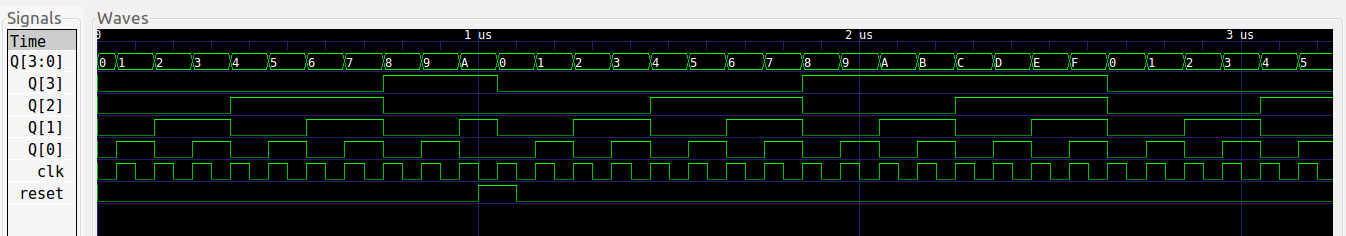
\includegraphics[width=\linewidth]{Waveform.png}
	%\label{fig:boat1}
\end{figure}

\begin{figure}[t]
	\caption{Pictures of the circuit}
	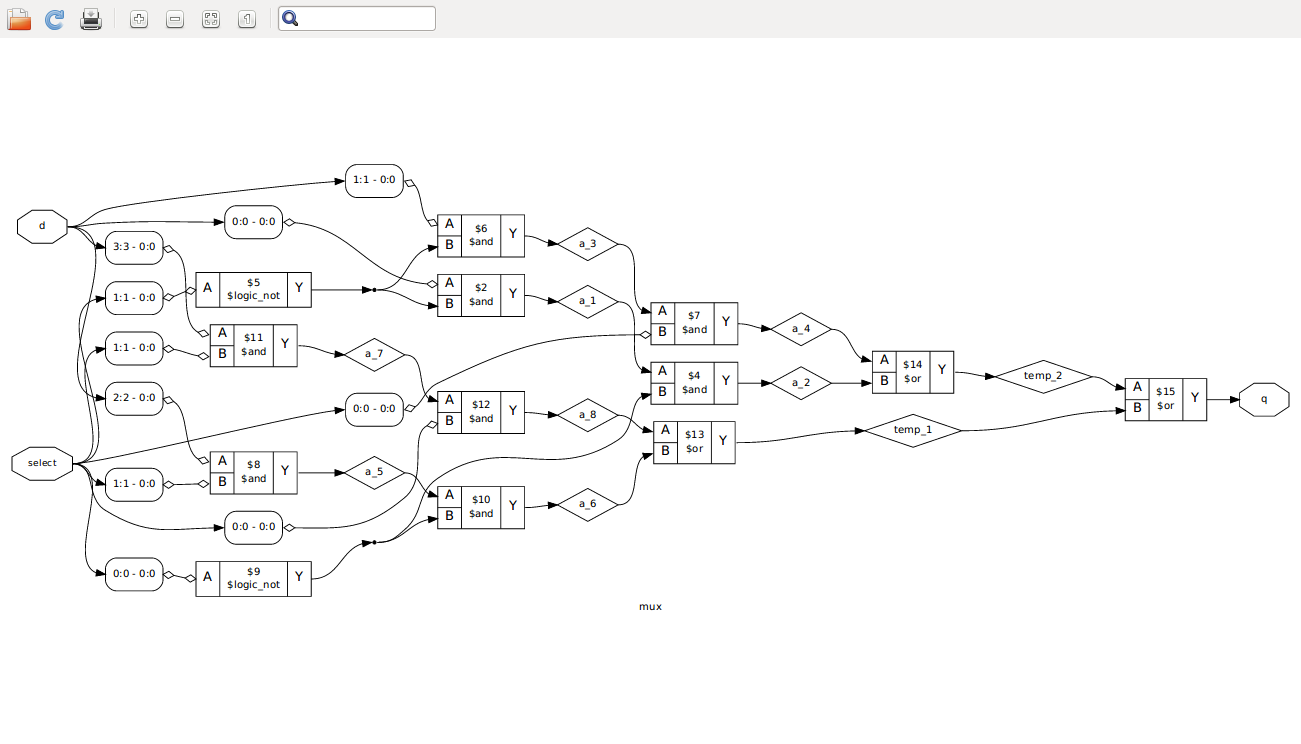
\includegraphics[width=\linewidth]{image.jpg}
	%\label{fig:boat1}
	
	
	\includegraphics[width=\linewidth]{another_one.jpg}
	%\label{fig:boat1}
\end{figure}

\section{Future Work}
\begin{itemize}
\item Increase the number of bits of the output using more registers.
\item Utilization of potentiometer to vary the speed of  counting.
\item Implementation of decoder to 7 segment display in hardware, and not using microcontroller.
\item Supplying clock signal without using a Arduino(ie. 555 timer circuit)

\end{itemize}


\section{Bibliography} 
\begin{itemize}
\item https://www.allaboutcircuits.com.

\item electronics-course.com/ripple-counter.

\item https://www.eecs.tufts.edu/~dsculley/tutorial

\end{itemize}
%----------------------------------------------------------------------------------------

\end{document}
